\documentclass[a4paper,11pt]{report} 
%\documentclass[8pt,twoside,twocolumn]{article}
%\documentclass[8pt,twoside]{article}
\usepackage[utf8]{inputenc} % Richtiges anzeigen von Umlauten und quasi allen anderen Schriftzeichen
\usepackage[T1]{fontenc} % Wichtig für alles was mehr als ASCII verwendet
%\usepackage[sc]{mathpazo} % Use the Palatino font
\usepackage{upgreek}
\usepackage{csquotes} % Schöne Anführungsstriche mit \enquote{Text}
\usepackage{amsmath} % Bessere und schönere mathematische Formeln
\usepackage{mathtools} % Noch schönerere mathematische Formeln
\usepackage{amstext} % \text{} Macro in mathematischen Formeln
\usepackage{amsfonts} % Erweiterte Zeichensätze für mathematische Formeln
\usepackage{amssymb} % Spezielle mathematische Symbole.
\usepackage{array} % Matrizen in mathematischen Formeln
\usepackage{textcomp} % Für textmu und textohm etc. um im Fließtext keine Mathematik 
\usepackage{textalpha} % Damit können griechische Zeichen direkt im Text verwendet werden (siehe zeichen.txt)
\usepackage{paralist} % Für compactitem und compactenum
\usepackage{braket} % Für das quantenmechanische Bra-Ket
%\usepackage{geometry} % Seitenränder und Seiteneigenschaften setzen
\usepackage[bottom]{footmisc} % Zwingt Fußnoten an das Ende der Seite
\usepackage[pdftex]{hyperref} % Links richtig anzeigen. Sowohl innerhalb des Dokuments (Fußzeilen, Formeln), als auch ins Internet
\usepackage[ % Biblatex für die Zitate und Referenzen
	backend=bibtex,
	hyperref=true
		]{biblatex}
\addbibresource{ref.bib}
\usepackage{graphicx} % Wichtig für das Einbinden von Grafiken
\usepackage{caption}
\usepackage{subcaption} % Einbinden von mehreren Grafiken in einer figure
\usepackage{float}
\usepackage{cleveref}
\usepackage{graphicx}  
\usepackage{txfonts}  
\usepackage{epstopdf}
\usepackage[miktex]{gnuplottex} % for MiKTeX,`pdflatex -shell-escape` enabled 
\usepackage{fancyhdr}
\usepackage[overload]{empheq}
\usepackage{ulem}
\usepackage{dsfont}
\usepackage{mathtools, cuted}
\usepackage{siunitx} % advanced unit package
\usepackage{titling}
%\usepackage[hmarginratio=1:1,top=10mm,left=12mm, right=12mm, bottom=18mm,columnsep=10pt]{geometry} % Document margins
%\usepackage[hmarginratio=1:1,left=28mm, right=28mm,]{geometry}
%\usepackage[hang, small,labelfont=bf,up,textfont=it,up]{caption} % Custom captions under/above floats in tables or figures
\usepackage{afterpage}
\usepackage{bm}
\usepackage[toc,page]{appendix}
\usepackage{titlesec}


\newcommand{\csubref}[2]{\namecref{#1}~\subref{#1:#2}}
%\renewcommand\thesection{\Roman{section}} % Roman numerals for the sections
%\renewcommand\thesubsection{\roman{subsection}} % roman numerals for subsections
%\titleformat{\section}[block]{\large\scshape\centering}{\thesection.}{1em}{} % Change the look of the section titles
%\titleformat{\subsection}[block]{\large}{\thesubsection.}{1em}{} % Change the look of the section titles
\titleformat{\chapter}{\normalfont\large\bf}{\thechapter.}{18pt}{\huge\bf}


\usepackage{abstract} % Allows abstract customization
\usepackage{blindtext} % Package to generate dummy text throughout this template

\usepackage{fontspec}
\newtheorem{theorem}{Theorem}
%\setmainfont{Verdana}

\renewcommand{\abstractnamefont}{\normalfont\bfseries} % Set the "Abstract" text to bold
\renewcommand{\abstracttextfont}{\normalfont\small\itshape} % Set the abstract itself to small italic

\newcommand*{\widebox}[2][0.5em]{\fbox{\hspace{#1}$\displaystyle #2$\hspace{#1}}}
\newcommand\eqquest{\mathrel{\overset{\makebox[0pt]{\mbox{\normalfont\tiny\sffamily ?}}}{=}}}
\newcommand{\pound}{\operatornamewithlimits{\#}}

\DeclareSIUnit{\calorie}{cal}
\DeclareSIUnit{\Calorie}{\kilo\calorie}
\sisetup{detect-all}

\captionsetup[figure]{font=small,labelfont=small}

\pagestyle{fancy}
\fancyhead{}
\fancyhead[L]{\small \leftmark}
\fancyhead[R]{\small \rightmark}

\hypersetup{ % Setzt einige Werte die in den Eigenschaften des PDF gespeichert sind.
	pdfauthor = {Klaus Steiner},
	pdftitle = {Topology},
	pdfdisplaydoctitle = true,
	colorlinks = false, % Für Druck auf "false" setzen!
} 

% Title Page
\pretitle{\begin{center}\huge\bfseries} % Article title formatting
\posttitle{\end{center}} % Article title closing formatting
\title{Topology in a correlated 2D system: a numerical analysis}
\author{Klaus Steiner}

%\renewcommand{\maketitlehookd}

\begin{document}
%\sffamily
\small
\maketitle

\begin{abstract}
//TODO: write abstract
\end{abstract}

\chapter{Introduction}\label{s:intro}

Topological materials are characterized by a nontrivial band structure with interesting properties. Usually the existence of edges is 
necessary to see the non trivial states in the band structure and allows to distinguish between the trivial bulk states and a number of non trivial
edge states which is also known as the bulk-edge correspondence. For a 2D topological insulator this results in an
insulating (interior) bulk states and conducting edge states.
The edge states can be identified as singular crossing bands near a symmetry point in the band structure. A fundamental requirement of these topological
phases are the existence or absence of symmetries. Depending which symmetry or symmetries and dimension apply to the system it falls into different topological 
classification with different edge state properties and characteristically topological indices or invariants. These invariants are based on the Berry 
phase and Berry curvature and should be explained briefly here. 

\section{Berry Phase and Berry Curvature}

We follow the derivations from \cite[p.7 - p.14]{Bernevig2013} here. Consider a system given by the Schrödinger equation
\begin{equation}
 \mathcal{H}(\bm{R}(t))\ket{n(\bm{R}(t)} = i\hbar\frac{d}{dt}\ket{n(\bm{R}(t)}
\end{equation}
for which the normalized eigenstates $\ket{n(\bm{R})}$ and eigenenergies $E_n(\bm{R})$ are known. The vector $\bm{R}$ represents a parameter set i.e 
position, electric field, magnetic field, strain etc. This system is now moved from time 0 to $t$ adiabatically. The only degree of freedom of the
state is the phase depending on time because according to the adiabatic theorem the state $\ket{n(\bm{R})}$ evolves with the Hamiltonian and only the
phase is arbitrary. By adding
explicitly a time depending phase $e^{-i\theta(t)}$ to the eigenstate in the Schrödinger equation, applying $\bra{n(\bm{R})}$ from left and solving it for the phase we get
\begin{equation}
 \theta(t) = \frac{1}{\hbar}\int_0^t dt^\prime E_n(\bm{R}(t^\prime)) 
 - i\int_0^t dt^\prime\braket{n(\bm{R}(t^\prime))|\frac{d}{dt^\prime}|n(\bm{R}(t^\prime))},
\end{equation}
where the first part is the conventional dynamic phase and the negative of the second part is the Berry phase. The differential operator in
the second part can be replaced by gradient operator $\nabla_{\bm{R}}$ due to the implicit time dependence of the parameter vector $\bm{R}$. Thus,
the Berry phase $\gamma_n$ can be written as
\begin{equation}\label{eq:1}
 \gamma_n = i\int_0^t dt^\prime\braket{n(\bm{R}(t^\prime))|\frac{d}{dt^\prime}|n(\bm{R}(t^\prime))} 
 = i\int_\mathcal{C} d\bm{R}\braket{n(\bm{R})|\nabla_{\bm{R}}|n(\bm{R})},
\end{equation}
Now, the $\gamma_n$ only depends on the curvature $\mathcal{C}$ in the parameter space and not explicitly on the time anymore. By defining the vector
potential $\bm{\mathcal{A}}_n(\bm{R}) \equiv \braket{n(\bm{R})|\nabla_{\bm{R}}|n(\bm{R})}$, \Cref{eq:1} can be rewritten as a curvature
integral of a vector potential
\begin{equation}\label{eq:2}
 \gamma_n = \int_\mathcal{C} d\bm{R}\cdot\bm{\mathcal{A}}_n(\bm{R})
\end{equation}
The vector potential $\bm{\mathcal{A}}_n(\bm{R})$ is not gauge invariant under the local transformation 
$\ket{n(\bm{R})} \rightarrow e^{i\chi(\bm{R})}\ket{n(\bm{R})}$ where $\bm{\mathcal{A}}_n(\bm{R})$ transforms as
\begin{equation}\nonumber
 \bm{\mathcal{A}}_n(\bm{R}) \rightarrow \bm{\mathcal{A}}_n(\bm{R}) - \nabla_{\bm{R}}\chi(\bm{R}).
\end{equation}
The function $\chi(\bm{R})$ is smooth along the curvature $\mathcal{C}$. On the other hand in the case of a closed curvature the Berry phase is 
indeed gauge invariant modulo $2\pi$. This can be seen by gauge transforming \Cref{eq:2} along a closed curvature
\begin{equation}
 \oint_\mathcal{C}d\bm{R}\cdot\bm{\mathcal{A}}_n(\bm{R}) \rightarrow \gamma_n 
 - \underbrace{\oint_\mathcal{C}d\bm{R}\cdot\nabla_{\bm{R}}\chi(\bm{R})}_{= 0}.
\end{equation}
The second term is zero because start and end point of the curvature are the same modulo $2\pi$. If the vector potential is smooth along a closed 
$\mathcal{C}$, the Stokes' theorem can be used to convert the curvature integral into a surface integral
\begin{equation}
 \oint_\mathcal{C}d\bm{R}\cdot\bm{\mathcal{A}}_n(\bm{R}) = \int_\mathcal{S}d\bm{S}\cdot\nabla_{\bm{R}}\times\bm{\mathcal{A}}_n(\bm{R})
 = \int_\mathcal{S}d\bm{S}\cdot\bm{\Omega}_n(\bm{R})
\end{equation}
where the definition $\bm{\Omega}_n(\bm{R}) \equiv \nabla_{\bm{R}}\times\bm{\mathcal{A}}_n(\bm{R})$ is used with $\bm{\Omega}_n(\bm{R})$
as the so called Berry curvature of the n-th eigenstate. 

\section{Invariants and Symmetries}

Based on the previous section we can define an integer number
\begin{equation}\label{eq:3}
 \nu \equiv \frac{1}{2\pi}\int_\mathcal{S}d\bm{S}\cdot\bm{\Omega}(\bm{R})
\end{equation}
which is called Chern number. To see that $\nu$ is an integer we can first start evaluating \Cref{eq:3} on a closed surface $\mathcal{S}$. By applying
again Stokes' theorem the integral converts back to an integral over the boundary $\partial \mathcal{S}$ which gives $\nu = 0$ because a closed 
surface has no boundary. But the previous argument requires that the vector potential $\bm{\mathcal{A}}(\bm{R})$ is smooth. Therefore, for a non trivial
Chern number a non smooth vector potential is crucial. In fact, a non trivial Chern number manifests that no gauge can be found for which 
$\bm{\mathcal{A}}(\bm{R})$ is smooth. In order to calculate the Chern number for a non smooth vector potential the integral in \Cref{eq:3} has to
be split up in piecewise smooth integrals or patches. Between the patches the vector potentials used in the integrals can be related through gauge
transformations and the resulting Chern number is then given by the sum of winding numbers of the gauge transformation along the 
surface of patches\cite[p.31]{Bernevig2013}.
As an example the Integer Quantum Hall Effect (IQHE) should be mentioned which was first discovered in 1975. On a 2-dimensional electron gas (i.e in the x-y plane)
a magnetic field perpendicular to the surface is applied. When applying an electric field in x-direction, a current $j_y$ in y-direction
can be measured resulting from the conductivity $\sigma_{xy} = \nu e^2/h$ which is quantized and proportional to the Chern number $\nu$. 
The parameter vector and the surface in \Cref{eq:3} are the magnetic field and
the Brillouin zone (BZ) respectively. In two dimension and periodic boundary condition the surface of the BZ becomes the one of a torus and is therefore
closed. Only the non trivial structure of the vector potential gives a non trivial Chern number. 

In this report we will focus on the 
Quantum Spin Hall Effect (QSHE). Compared to the IQHE where the system has no symmetry, for a QSHE breaking the time reversal
symmetry is crucial. In detail
\begin{equation}
 \left[\mathcal{H}, \mathcal{T}\right] = 0 \Rightarrow \mathcal{H} = \mathcal{T}\mathcal{H}\mathcal{T}^{-1} \xrightarrow{\mathrm{F.T}}
 \mathcal{H}_{-k} = \mathcal{T}\mathcal{H}_{k}\mathcal{T}^{-1}.
\end{equation}
The time reversal operator $\mathcal{T}$ is an anti-unitary operator and can be composed as $\mathcal{U}\mathcal{K}$ where $\mathcal{U}$ is an unitary
operator and $\mathcal{K}$ complex conjugation. In a spin system $\mathcal{U}$ is responsible for flipping the spin and $\mathcal{K}$ changing momentum
$\bm{p}$ to $-\bm{p}$. Due to the anti-unitary, $\mathcal{T}^2$ can only take the values $\pm 1$. In the case of a Fermionic 
system invariant under $\mathcal{T}$, $\mathcal{T}^2$ is $-1$ and the Kramer's theorem holds: 
\begin{theorem}[Kramer's theorem]
For any eigenstate $\ket{\psi}$ and energy $E$ of a 
time reversal fermionic system, there exists another state $\mathcal{T}\ket{\psi}$ with the same energy $E$.
\end{theorem}
This degeneracy will play an important role in calculating the $\mathds{Z}_2$ number, which is the topological invariant for nonmagnetic systems. 
For an eigenstate $\ket{\bm{k}}$ the degenerate state is 
$\mathcal{T}\ket{\bm{k}} = \ket{-\bm{k}}$ with different momentum. But for $\ket{\bm{k} = 0}$ the time reversed state $\mathcal{T}\ket{\bm{k} = 0}$
is a different state with the same energy and momentum. This i.e also applies for $\ket{\bm{k} = (0,\pi)}$ in a two dimensional k-grid where
$\mathcal{T}\ket{\bm{k} = (0,\pi)} = \ket{\bm{k} = (0,-\pi)}$ is the same state. These particular points need to be treated different in the
method described in \Cref{s:methods}. 

The Kramer's theorem is also responsible for the topological protection of the edge state against small
perturbation. The well-known Kane-Mele model (see \Cref{s:methods}) includes a spin-orbit coupling perturbation where the edge states remain
topological.

A more general classification of topological states of matter can be achieved with the ten-fold classification based on three symmetry operation types. For
the QSHE we already mentioned the breaking of time reversal symmetry which is in a more general definition a anti-unitary operation. If we also include
unitary and chiral operators (unitary operator which anti commutes with the Hamiltonian) we can build upon this a table with the relevant topological invariant for a particular dimension. For a given system with
a second quantized Hamiltonian $\hat{\mathcal{H}}$, we can separate it in the following way:
\begin{equation}\label{eq:7}
 \hat{\mathcal{H}} = \hat{\psi}^{\mathrm{T}}\mathcal{H}\hat{\psi}
\end{equation}
where the $\hat{\psi}^{\mathrm{T}}$ and $\hat{\psi}$ are vectors of creation and annihilation operators respectively. This means, that in order to
investigate a system, we only have to look at $\mathcal{H}$ and which doesn't necessarily need to be a quantum mechanical system.
The system described with Hamiltonian operator $\mathcal{H}$ has to fulfills one or more of the above symmetries criteria.

In the Kane-Mele model perturbation in terms of a spin orbit coupling is included where we still find the topological states.\\
\\
//TODO: make reference to self energy and what' the purpose of this report (topology with correlation)


\chapter{Methods}\label{s:methods}

All Results are generated by a program written in C++. The program is based on a older version and was extended to achieve a more flexible
configuration and extendability and more important to include self energy. The Hamiltonian used by the program is calculated through the tight binding model (see \Cref{a:tb}).
It takes as program argument a goal, which defines the computation algorithm and the corresponding output it should
generate and a configuration file which contains the tight-binding Hamiltonian, grid, k-path, etc. For a more detailed explanation see \Cref{a:program}.

\section{Kane-Mele Model}\label{s:kane-mele}

The Kane-Mele model is a honeycomb lattice model which also takes spins into account. It is based on the Haldane model which is a tight binding model
having a nearest neighbor and a complex next nearest neighbor hopping. The honeycomb lattice consists of two lattice sites A and B where nearest
neighbor hopping $t_1$ couples A to B and the complex next nearest neighbor hopping operates between same lattice sites (see \Cref{f:honeycomb}).
The complex next nearest
neighbor hopping comes in the Hamiltonian through a phase $\phi$, where from A to B the phase is positive and from B to A negative. The full Hamiltonian in
real space is
\begin{equation}\label{eq:4}
 \hat{\mathcal{H}}^{\mathrm{Haldane}} = t_1\sum_{<i,j>}a_i^\dagger b_j + t_2\sum_{<<i,j>>}\left(e^{i\phi}a_i^\dagger a_j + e^{-i\phi}b_i^\dagger b_j\right)
 + M\sum_{i}\left(a_i^\dagger a_i - b_i^\dagger b_i\right)
\end{equation}
where the first sum is nearest neighbor hopping, the second term the next nearest neighbor hopping (breaks time reversal symmetry) and the last term 
the on-side energy difference (breaks the inversion symmetry). The $a_i^\dagger$/$b_i^\dagger$ and $a_i$/$b_i$ are the creation and annihilation operators for lattice side
A/B on grid point $i$ respectively. We extend this Hamiltonian to include spin up and down\cite{Kane2005}. For the non interacting part of the Hamiltonian we can simply
copy the terms of \Cref{eq:4} for both spin up and down. Only the next nearest neighbor term looks a bit different.
\begin{equation}\label{eq:5}
\begin{split}
 \hat{\mathcal{H}}_0^{\mathrm{KM}} &= t_1\sum_{<i,j>,\bm{s} = \uparrow\downarrow}a_{i,\bm{s}}^\dagger b_{j,\bm{s}} 
 + M\sum_{i, \bm{s} = \uparrow\downarrow}\left(a_{i,\bm{s}}^\dagger a_{i,\bm{s}} - b_{i,\bm{s}}^\dagger b_{i,\bm{s}}\right)\\ 
 &+ t_2\sum_{<<i,j>>}\left(e^{i\phi}a_{i,\uparrow}^\dagger a_{j,\uparrow} + e^{-i\phi}b_{i,\uparrow}^\dagger b_{j,\uparrow}\right)\\ 
 &+ t_2\sum_{<<i,j>>}\left(e^{-i\phi}a_{i,\downarrow}^\dagger a_{j,\downarrow} + e^{i\phi}b_{i,\downarrow}^\dagger b_{j,\downarrow}\right).
\end{split}
\end{equation}
\begin{figure}[H]
\begin{center}
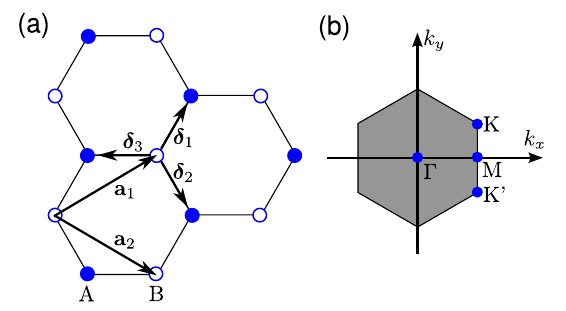
\includegraphics[scale=0.50]{figures/honeycomb}
\caption{(a) Honeycomb lattice\cite{Hohenadler2013} with nearest ($\delta_i$) and next nearest neighbors ($a_i$). (b) The unit cell with the
symmetry points $\Gamma$, K and K'}
\label{f:honeycomb}
\end{center}
\end{figure}
\Cref{eq:5} is invariant under time reversal without giving a proof here. So far, we did not couple electrons with different spins. The goal is to add
spin coupling terms while keeping the time reversal symmetry. As long we keep time reversal symmetry the Kramer's theorem hold and we obtain
protected edge states visible as crossing bands in the band structure. To see what happens when we add perturbation to the system we can write the
Kane-Mele Hamiltonian in the following form
\begin{equation}
  \hat{\mathcal{H}}^{\mathrm{KM}} = \left(\begin{matrix}\hat{\psi}_{\uparrow} & \hat{\psi}_{\downarrow}\end{matrix}\right)\left(\begin{matrix}
\mathcal{H}^{\mathrm{Haldane}}(\phi)  & J^\dagger\\
 J & \mathcal{H}^{\mathrm{Haldane}}(-\phi)& 
\end{matrix}\right)\left(\begin{matrix}\hat{\psi}_{\uparrow} \\ \hat{\psi}_{\downarrow}\end{matrix}\right)
\end{equation}
which is the same separation as in \Cref{eq:7}. The off-diagonal block $J$ is the coupling with the constraint to be anti-symmetric, so $J^{\mathrm{T}} = -J$. Every coupling which flips spins
and is anti-symmetric is allowed and fulfills time reversal symmetry. Again, we show no proof here. A possible coupling which satisfies the requirements
is the Rashba spin-orbit coupling.

\section{Input Data}

For the tight-binding model the input is generated through a DFT + Wannier projection with the Wien2k and Wien2Wannier package.The resulting output
after wannierization contains the unit cell structure, neighbor indices, atom indices and the real and imaginary hopping or orbital overlap.
The program takes this input and generates a matrix out of it, based on the used boundary conditions. Due to spin-orbit coupling resulting from
DFT is very small, we increased it to make it more visible in the band structure. \Cref{fig:bs}\subref{fig:GMKG-1px1p} and 
\Cref{fig:bs}\subref{fig:GMKG-1px1p-soc}
shows the band structure of graphene with and without a spin-orbit
coupling.
The self energy can given as input file, set to a constant value or the analytic form
\begin{equation}\label{eq:10}
 \Sigma(\omega) = \frac{U^2}{4}\frac{\omega - i\delta}{\omega^2 + \delta^2}
\end{equation}
can be used which is the atomic limit for the insulating case. Graphene consists of C atoms in a $sp^2$ hybridization state. Due to this
hybridization there are only two bands in \Cref{fig:bs} $\pi$ where each band is degenerated by 2. Every C atom contributes one $\pi$ electron
and occupies the lowest band with one spin up and one spin down electron (the unit cell consists of 2 atoms). In the literature the lower and
upper bands are often symmetric compared to the band structure in \Cref{fig:bs}. This is because we included also next nearest neighbor hopping
in the tight-binding Hamiltonian which makes the band structure look asymmetric. 

\section{Spectral Function}

//TODO: finish this section and make it better\\\\
In order to investigate the behavior of the bands and the topological states when including correlation through self energy we are calculating the 
spectral function
\begin{equation}
 A(\omega,\bm{k}) = -\frac{1}{\pi}\mathrm{Im}G(\omega,\bm{k}).
\end{equation}
where $G(\omega,\bm{k})$ is the Green's function.
The program provides three different options for calculation:
\begin{enumerate}
 \item k-resolved spectral function
\end{enumerate}

\section{$\mathds{Z}_2$ Calculation}\label{s:z2}

For a QSHE system the Chern number is always zero because in every pair of double degenerate bands both constitutes have opposite Chern number,
hence their sum is zero. There is a different characteristic
invariant called $\mathds{Z}_2$, which can only be 0 or 1 depending if it is topological or not. This invariant is connected to the so called
pfaffian
\begin{equation}
 P(\bm{k}) = Pf\left\{\braket{n(\bm{k})|\mathcal{T}|m(\bm{k})}\right\}.
\end{equation}
The absolute value of pfaffian $\left|P(\bm{k})\right|$ is gauge invariant and only 0 or 1. It turns out that an odd number of zero pfaffians is
a topological non trivial system. In order to calculated the $\mathds{Z}_2$ invariant the space spanned
by the eigenstates $\ket{n(\bm{k})}$ is divided into an even and odd subspace. The even subspace are all eigenstates which follows the constraint
\begin{equation}
 \mathcal{T}\ket{n(\bm{k})} =  M_{nm}\ket{m(\bm{k})}
\end{equation}
and therefore all k-points satisfying $\mathcal{T}\mathcal{H}(\bm{k})\mathcal{T}^{-1} = \mathcal{H}(-\bm{k}) = \mathcal{H}(\bm{k})$. In graphene the
$\gamma$ and the $M$ points are such time reversal invariant points (TRIM). $M_{nm}$ is a
matrix containing only off-diagonal elements. The odd subspace are all states for which
\begin{equation}
 B_{mn}(\bm{k})\mathcal{T}\ket{n(\bm{k})} = \ket{n(-\bm{k})}
\end{equation}
holds and where $\mathcal{T}\mathcal{H}(\bm{k})\mathcal{T}^{-1} = \mathcal{H}(-\bm{k}) = -\mathcal{H}(\bm{k})$. $B_{nm}(\bm{k})$ is an unitary matrix
called sewing matrix. Kane and Mele showed that there is a binary invariant which can be calculated through
\begin{equation}\label{eq:8}
 I = \frac{1}{2\pi i}\oint_{\mathcal{C}} d\bm{k} \nabla_{\bm{k}}\log{\left(P(\bm{k}) + i\delta\right)}
\end{equation}
where $\mathcal{C}$ is now a curvature around the half of the Brillouin zone and $\delta$ a convergence factor. $I$ itself depends on the gauge and
the sign of $\delta$ but $I$ modulo 2 is indeed invariant. \Cref{eq:8} counts the number of complex zeros pairs of $P$. These zeros of the pfaffian are
topological invariant. If there is a odd number of zero pfaffian we have a topological system. An alternative form of the $\mathds{Z}_2$ calculation is
\begin{equation}\label{eq:9}
 I = \frac{1}{2\pi i}\oint_{\partial\mathcal{B}^-}d\bm{k}\mathcal{A}_i(\bm{k}) - \int_{\mathcal{B}^-}d\bm{k}\mathcal{F}_{ij}(\bm{k}) 
\end{equation}
where $\mathcal{B}^-$ denotes know the half BZ and $\mathcal{F}_{ij}(\bm{k})$ is in analogy to electro dynamics the field strength.
%composed from $\mathcal{\bm{A}}(\bm{k})$ as $\mathcal{F}_{ij}(\bm{k}) = \partial_i\mathcal{A}_j(\bm{k}) - \partial_j\mathcal{A}_i(\bm{k})$
\begin{figure}[H]
\begin{center}
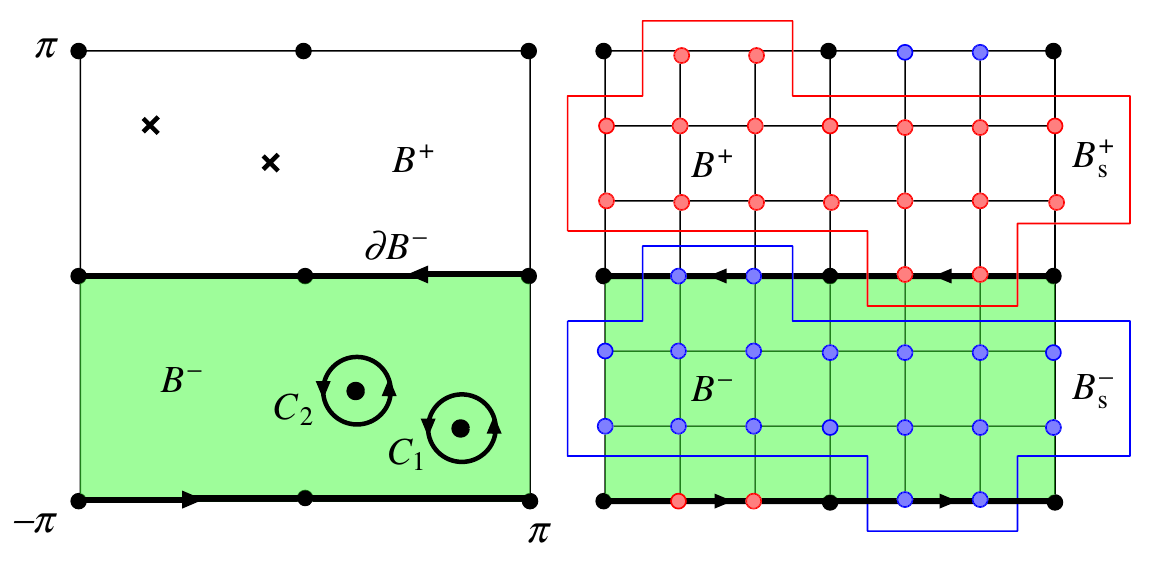
\includegraphics[scale=0.30]{figures/k-space-z2}
\caption{The k-space for the $\mathds{Z}_2$ calculation for the method developed by Fukui and Hatsugai\cite{Fukui2007}. The space is divided in $\emph{B}^-$  and
 $\emph{B}^+$ where only $\emph{B}^-$ is used for calculation. The black dots are the TRIMs, $\emph{B}_\mathrm{S}^-$ are points of the odd
 space and the black line is the boundary of half the Brillouin zone.}
\label{f:k-space-z2}
\end{center}
\end{figure}
Fukui and Hatsugai\cite{Fukui2007} build upon this a numerical version for a discrete k-space. $\mathcal{A}_i$ and $\mathcal{F}_{ij}$ are then calculated through
a link variable by
\begin{subequations}\label{eq:11}
 \begin{align}
  U_i(\bm{k}_n) &= \frac{\det\left(\psi^\dagger(\bm{k}_n)\psi(\bm{k}_n 
  + \hat{i})\right)}{\left|\det\left(\psi^\dagger(\bm{k}_n)\psi(\bm{k}_n + \hat{i})\right)\right|}\\
  \mathcal{A}_i(\bm{k}_n) &= \ln{U_i(\bm{k}_n)}\\
  \mathcal{F}_{ij}(\bm{k}_n) &= \ln{\left[U_i(\bm{k}_n)U_j(\bm{k}_n + \hat{i})U_i^{-1}(\bm{k}_n + \hat{j})U_j^{-1}(\bm{k}_n)\right]}
 \end{align}
\end{subequations}
where $U_i$ is the link variable in direction $\hat{i}$, $\psi$ is a $2\times2$ matrix spanned by the degenerated eigenvectors for spin up and down,
$\bm{k}_n$ denotes the nth k-point in the grid. For a two dimensional grid $\hat{i}$ and $\hat{j}$ are the two canonical basis vectors in two dimensions
respectively. The lattice version of \Cref{eq:9} for two dimensions is then given by
\begin{equation}
 I_{\mathrm{L}} = \frac{1}{2\pi i}\left[\sum_{\bm{k}_n \epsilon \partial \mathcal{B}^{-}}\mathcal{A}_1(\bm{k}_n) 
 - \sum_{\bm{k}_n \epsilon \mathcal{B}^{-}} \mathcal{F}_{12}(\bm{k}_n)\right] 
\end{equation}
with the result as an integer and modulo 2 the $\mathds{Z}_2$ number. The previous calculations can be extended also in 3 dimensions. If we consider
the Brillouin zone as a cube we have 6 different surfaces where each of the surface represents a torus due to periodic boundary conditions. This means
we fix on coordinate of the $\bm{k}$-vector either to 0 or $\pi$ (to include the TRIMS) and obtain these 6 different possibilities. 
We follow \cite{Fukui2007} and denote the invariants of the surfaces
as $x_0$ if $k_x = 0$ or $x_\pi$ if $k_x = \pi$ and in the same way $y_0$, $y_\pi$, $z_0$ and $z_\pi$. It turns out that in three dimension only 4 
$\mathds{Z}_2$ invariants denoted as $I_0(I_1;I_2;I_3)$ are independent because there are the constraints $x_0\cdot x_\pi = y_0\cdot y_\pi = z_0\cdot z_\pi$.
Without any loose of generality we can fix the invariants to $I_0 = x_0\cdot x_\pi$ and $I_1 = x_\pi$, $I_2 = y_\pi$ and $I_3 = z_\pi$.

\section{Chern Number Calculation}

We mention here briefly the calculation of Chern number for the discrete case. It is very similar to the method described in \Cref{s:z2} and taken from
\cite{Fukui2008}. Compared to the $\mathds{Z}_2$ calculation where the Berry vector potential is non-Abelian because $\psi$ in \Cref{eq:11} is a $2\times 2$
matrix with $U_i$ as the normalized overlap of the multiplet states, we can define the definition for $U_i$ in \Cref{eq:11} for a spin-less system as
\begin{equation}
  U_i(\bm{k}_l) = \frac{\braket{n(\bm{k}_l)|n(\bm{k}_l + \hat{i})}}{\left|\braket{n(\bm{k}_l)|n(\bm{k}_l + \hat{i})}\right|}.
\end{equation}
In analogy to \Cref{s:z2} the lattice version for Chern number is given by
\begin{equation}
 \nu_{\mathrm{L}} = \frac{1}{2\pi i}\sum_l\mathcal{F}_{12}(\bm{k}_l)
\end{equation}
where $\mathcal{F}_{12}$ is again the field strength and the same definition as in \Cref{eq:11}.

\chapter{Results}\label{s:results}

As in the previous chapters mentioned, we are interested in studying the edge states of the topological material under adding correlation through
self energy. We are interested in the QSHE based on the Kane-Mele model described in \Cref{s:kane-mele}.
\begin{figure}[H]
\centering
\begin{subfigure}{.49\textwidth}
  \centering
  \includegraphics[width=1.0\linewidth]{../../results/bs/GMKG_1px1p.png}
  \label{fig:GMKG-1px1p}
  \caption{}
\end{subfigure}
\begin{subfigure}{.49\textwidth}
  \raggedleft
  \includegraphics[width=1.0\linewidth]{../../results/bs/GMG_1px50o.png}
  \label{fig:GMG-1px50o}
  \caption{}
\end{subfigure}
\begin{subfigure}{.49\textwidth}
  \centering
  \includegraphics[width=1.0\linewidth]{../../results/bs/GMKG_1px1p_soc.png}
  \label{fig:GMKG-1px1p-soc}
  \caption{}
\end{subfigure}
\begin{subfigure}{.49\textwidth}
  \raggedleft
  \includegraphics[width=1.0\linewidth]{../../results/bs/GMG_1px50o_soc.png}
  \label{fig:GMG-1px50o-soc}
  \caption{}
\end{subfigure}
\caption[]{Bandstructure calculations for graphene with and without a SOC and periodic and open boundary conditions (BC). The blue lines are the bulk
 states and the red the edge states. (a) Periodic BC and no SOC,
 (b) One direction with open BC and no SOC, (c) Periodic BC and SOC, (d) One direction with open BC and SOC}
\label{fig:bs}
\end{figure}
First we verified our model by plotting the band structure of graphene. For the the three dimensional k-path $\Gamma$ - M - K - $\Gamma$ in
\Cref{fig:bs}a and \Cref{fig:bs}c we calculated the bandstructure with periodic boundary conditions without and with a spin-coupling (SOC).
As expected a gap opens for the case with SOC at the K-point.
The next step was to make the bulk finite by applying an open boundary
condition in one direction and calculate the bandstructure for the one dimensional k-path $\Gamma$ - M - $\Gamma$ in Zig-Zag direction. \Cref{fig:bs}b 
and \Cref{fig:bs}d show the results with a bulk consisting of 50 unit cells. Again we included and excluded SOC. The K2-points in this figures is the projection of
the K-point in the one dimensional k-path and therefore, the point where the gap opens when adding SOC. The M-point is the important point
where the crossing of the edge states occurs. As explained in \Cref{s:kane-mele} the M-point is a TRIM point for which Kramer's theorem holds
and the edge states are topological protected. This topological protected can be tested out by adding energy to the edge states and shifting them towards
higher energies. If the edge states are shifted over the band gap the next unit cells are taking over as topological states and therefore Kramer's
theorem is not violated. This can be seen in \Cref{f:resw}
\begin{figure}[H]
\centering
\begin{subfigure}{.49\textwidth}
  \centering
  \includegraphics[width=1.0\linewidth]{../../results/bs/GMG_1px50o_resw.png}
  \label{f:GMG_1px50o_resw}
  \caption{Without SOC}
\end{subfigure}
\begin{subfigure}{.49\textwidth}
  \raggedleft
  \includegraphics[width=1.0\linewidth]{../../results/bs/GMG_1px50o_soc_resw.png}
  \label{f:GMG_1px50o_soc_resw}
  \caption{With SOC}
\end{subfigure}
\caption{Bandstructure plots when adding real self energy of 10 units at the edge.}
\label{f:resw}
\end{figure}
Now we include correlation through a self energy $\Sigma(\omega)$ where we distinguish between a metallic and an insulating self energy. In the case
of atomic limit, $\Sigma(\omega)$ can be calculated analytical and takes the form in \Cref{eq:10}, so $\propto \frac{1}{\omega}$. 
\begin{figure}[H]
\centering
\begin{subfigure}{.49\textwidth}
  \centering
  \includegraphics[width=1.15\linewidth]{../../results/awk/insu_insu/step3.png}
  \label{fig:insul-insul}
  \caption{Insulating self energy on edge and bulk with $U = 3$}
\end{subfigure}
\begin{subfigure}{.49\textwidth}
  \raggedleft
  \includegraphics[width=1.15\linewidth]{../../results/awk/insu_metal/step19.png}
  \label{fig:insul-metal}
  \caption{Insulating self energy in bulk with $U = 19$ and metallic self energy on edge.}
\end{subfigure}
\begin{subfigure}{.49\textwidth}
  \centering
  \includegraphics[width=1.15\linewidth]{../../results/awk/metal_metal/metal_metal.png}
  \label{fig:metal-metal}
  \caption{Metallic self energy in bulk and on edge.}
\end{subfigure}
\begin{subfigure}{.49\textwidth}
  \raggedleft
  \includegraphics[width=1.15\linewidth]{../../results/awk/metal_insu/step19.png}
  \label{fig:metal-insul}
  \caption{Metallic self energy in bulk and insulating self energy with $U = 19$ on edge.}
\end{subfigure}
\caption[]{Spectral function plots for different analytical self energies in bulk and on edge.}
\label{fig:awk}
\end{figure}
\Cref{fig:awk}\subref{fig:insul-insul} to \Cref{fig:awk}\subref{fig:metal-insul} show the spectral function plots with
different $U$ values. For the case with insulating bulk and edge an increasing $U$ separates the lower and upper Hubbard
bands. The two valence bands around the Fermi energy are getting thinner with lower $U$ due to a pole at zero energy
which forces the squeezing of the bands. For metallic self energy on edge, insulating self energy in bulk and $U$ bigger 
than the band gap, the crossing bands in \Cref{fig:awk}\subref{fig:insul-metal} are resulting from a one dimensional
chain created by the boundary conditions. Except of the one dimensional chain bands the plot is the same as 
\Cref{fig:awk}\subref{fig:insul-insul} only with higher $U$. In the case of insulating edge and metallic bulk the resulting
spectral function plot is \Cref{fig:awk}\subref{fig:metal-insul}. As it can be seen, the insulating self energy shifts out 
the edge states but the system remains topological.

%TODO: 
% *) for the metal-insul case, take step19 where it is clearly visible that it is remaining topological
%    and only edge is only shifted out and the next layer overtakes.
% *) for metal-metal it is clear what happens.
% *) for insul-insul case: explain with the pole in the middle and the seperation of the states where the small bands
%    in the middle are the previous valence bands.
% *) for the insul-metal case: show that the bands when U is high (i.e 19) it is only a one dimensional chain. For lower
%    U where the chain states are touching the valence bands there is also something in between the band gap. ask Oleg

\chapter{Conclusion}

\appendix

\chapter{Tight Binding Model}\label{a:tb}
\chapter{Program}\label{a:program}

The program was written in a modern C++ and focuses on easy extendability for adding new calculation routines by defining new models and quantities
in the source code. The basis is the
tight-binding model and the program requires a Hamiltonian file as input and also the dimension and boundary conditions of
the system. This can be configured in the configuration file described in \Cref{s:config-file}. The code of the program can
handle arbitrary dimensions but currently only dimensions from 1 to 3 are implemented. This is possible through the generic
design pattern where the dimension of the system is given as template class parameters. To start a calculation, the program 
needs as argument a goal which is the model name it should evaluate and the path to the configuration file. A third parameter
is optional and is the path to the output file. If no output file is specified the standard output stream is used. This could
be useful if the whole program output including calculation results should be piped into one file. 

\section{Configuration File}\label{s:config-file}

The configuration file has a JSON-like/C-like style which allows to define also nested structures. The file must contain a path
to the tight-binding Hamiltonian in Wannier90 format and information about dimension and boundary conditions. Depending which
model is called different additional configurations are required. An example of the mandatory configuration blocks is given below
which every valid configuration has to include. The Hamiltonian is read from the file \texttt{graphene.dat} and a 2 dimensional 
system with open and periodic boundary conditions and size $1\times50$ in units of unit cells is defined.
\lstset{language=C++,
                basicstyle=\fontsize{8}{8}\ttfamily,
                keywordstyle=\color{blue}\ttfamily,
                stringstyle=\color{red}\ttfamily,
                commentstyle=\color{green}\ttfamily,
                morecomment=[l][\color{magenta}]{\#}
                backgroundcolor=\color{gray},
                language=C
}
\begin{lstlisting}[frame=single] 
/**
 * Tight-Binding Hamiltonian (mandatory)
 * -------------------------------------
 * this must be a valid file path
 */
 hr = "graphene.dat";
 
/**
 *       Real Space Grid (mandatory)
 * --------------------------------------
 * Here the dimension and size of the system are defined.
 * Currently dimensions from 1 - 3 are supported and have
 * the names x, y and z respectively. For every direction
 * the size dim and the boundary condition bc can be
 * specified.
 */
rgrid = {
    x = {\pm
        dim = 1;
        //periodic boundary condition
        bc = "p";
    }
    y = {
        dim = 50;
        //open boundary condition
        bc = "o";
    }
}
\end{lstlisting}
In the same way \texttt{C/C++} does not require line breaks and tabulators because these are only formatting characters, the
syntax also requires only semicolons for assignments endings and curly brackets to enclose object definitions.
The keywords in the given example are defined in the code and must be matched if new configurations are made. Some models
need as input a k-path. This can be defined in the following way
\begin{lstlisting}[frame=single] 
 ...
 /**
 *           k-Path (optional)
 * --------------------------------------
 * Again here are different options possible:
 * (1) input file. The program supports paths created
 * with xcrysden.
 * (2) defining symmetry points and the path between
 * those. Here the 'dens' parameter are the number of
 * points between two symmetry points. The 'path' parameter
 * defines the path. Every symmetry point is defined as
 * an object with parameters kx, ky and kz. The default value
 * for these is zero, so if some of these are not defined
 * there are set to zero.
 */
//kpath = "...";    // option (1)
kpath = {           // option (2)
    dens = 100;
    path = "G-M-G";
    G = {
        kx = 0;
        ky = 0;
        kz = 0;
    }
    M = {
        kx = 1/2;
        ky = 0;
        kz = 0;
    }
    Q = {
        kx = 1/3;
    }
}
\end{lstlisting}
The \texttt{kpath} keyword can either be set to a file path in format of the xcrysden k-path
file format or a path can be defined by symmetry points and a density factor. In a similar way
a self energy input can be defined
\begin{lstlisting}[frame=single] 
/**
 *      Bulk Self Energy (optional)
 * -------------------------------------
 *  (1) This can be either a path to a file
 * where the file must have the follwing colums:
 * # energy | Re(sigma) 1 | Imag(sigma) 1 | | Re(sigma) 2 | Imag(sigma) 2 | ...
 *   ...
 * where the numbers in the names denote the atoms. So for every atome there
 * is one real and imaginary self energy value.
 * (2) Self
 */
//sw = "...";       // option (1)
sw = {              // option (2)
    dens = 1000;
    w_min = -12;
    w_max = 12;
    U = 1;
    delta = 0.01;
    sigma = "iso";    // example for sub option (1)
    //sigma = -0.01i  // example for sub option (2)
}
\end{lstlisting}
Currently supported models are 
\begin{enumerate}
 \item \text{Bandstructure} \texttt{--goal bs}
 \item \text{Density of States} \texttt{--goal dos}
 \item \text{Spectral Function} \texttt{--goal Aw/Awk/AwEdge}
 \item \text{Chern Number} \texttt{--goal chern}
 \item \text{Z2 Invariant} \texttt{--goal Z2}
\end{enumerate}


\subsection{}



\section{Extending the Code}

\printbibliography

\end{document}
